\documentclass{elsarticle}

\usepackage{amsmath}


\begin{document}

\begin{frontmatter}
\author{Ashwin Srinath}
\title{A}
\maketitle

\begin{abstract}
    We present a computation strategy for evaluating
    compact finite differences efficiently on GPU clusters.
    We describe a novel algorithm for solving the
    near-Toeplitz tridiagonal systems associated with
    the compact finite difference schemes.
    Our specialized tridiagonal solver
    takes advantage of the near-Toeplitz nature of the
    tridiagonal system to precompute the coefficients
    appearing in the Cyclic Reduction algorithm.
    This allows us to solve the tridiagonal systems
    up to 2 times faster than with the NVIDIA CUSPARSE
    gtsvStridedBatch routine.
    Additionally, we present a methodology to solve for
    compact finite differences fully on multiple GPUs on a cluster
    without intermediate host-device transfers.
\end{abstract}

\end{frontmatter}
    
\section{Introduction}

\section{Related work}
      
\section{Compact Finite Difference Schemes}

For example,
in a uniformly spaced one-dimensional grid with spacing $dx$,
if $f_i$ represents the value of
the function evaluated at the $i$th node,
the first derivative $f^{\prime}_i$ can be approximated from
a relation of the form:

\begin{equation}
\begin{split}
    \beta(f^{\prime}_{i-2} + f^{\prime}_{i+2}) + \
    \alpha(f^{\prime}_{i-1} + f^{\prime}_{i+1}) + \
        f^{\prime}_i
    = 
    c\frac{f_{i+3} - f_{i-3}}{dx} + \
    b\frac{f_{i+2} - f_{i-2}}{dx} + \\
    a\frac{f_{i+1} - f_{i-1}}{dx} + \
    \hdots
\end{split}
\label{eqn:general-compact}
\end{equation}

The derivatives near the boundaries are approximated using
one-sided stencil operators of the form:

\begin{equation}
f^{\prime}_1 + \alpha_1 f^{\prime}_2 = \
    \frac{1}{dx} (a_1 f_1 + b_1 f_2 + c_1 f_3 + d_1 f_4) 
\end{equation}

and 

\begin{equation}
    f^{\prime}_n + \alpha_n f^{\prime}_{n-1} = \
    \frac{1}{dx} (a_n f_n + b_n f_{n-1} + c_n f_{n-2} + d_n f_{n-3}) 
\end{equation}

As described by Lele \cite{lele1992compact},
setting $\beta = 0$ in Equation \ref{eqn:general-compact} leads to
a family of tridiagonal schemes with a single parameter ($\alpha$).
The coefficient matrix associated with such tridiagonal schemes
has the general form:

\begin{equation} \label{eqn:compact-tridiagonal-system}
\begin{bmatrix}
     1 &  \alpha_1  \\
     \alpha   &  1   &  \alpha \\
         &  \alpha   &  1  &  \alpha  \\
         &      &  \alpha  &  1  &  \alpha  \\
         &      &     &     &  \ddots \\
         &      &     &     &     &  \ddots  \\
         &      &     &     &     &  \alpha_n &  1
\end{bmatrix}
\begin{bmatrix}
    f^{\prime}_1 \\
    f^{\prime}_2 \\
    f^{\prime}_3 \\
    \vdots \\
    \vdots \\
    f^{\prime}_{n-1} \\
    f^{\prime}_n
 \end{bmatrix}
=
\begin{bmatrix}
   d_1 \\
   d_2 \\
   d_3 \\
   \vdots \\
   \vdots \\
   d_{n-1} \\
   d_{n}
\end{bmatrix}
\end{equation}

We note that the system is \emph{near Toeplitz tridiagonal},
i.e., the left-hand-side matrix is tridiagonal with
constant coefficients along each diagonal,
except for the first and last equations.

\section{Evaluation of compact finite differences}

\begin{figure}[h!]
\begin{center}
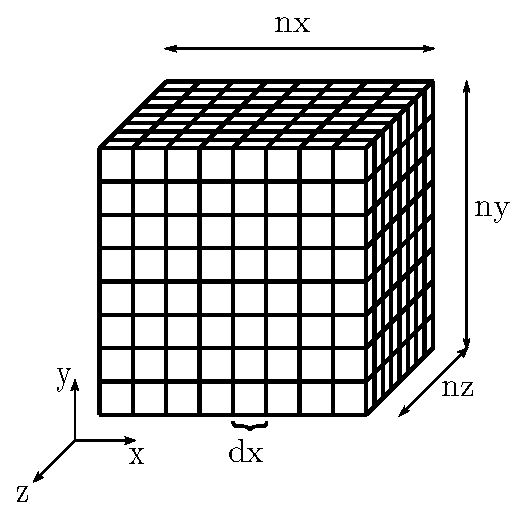
\includegraphics[height=200pt]{img/computational-domain.eps}
\end{center}
\caption{Computational domain in 3-D}
\label{fig:computational-domain}
\end{figure}

The computational domain (Figure \ref{fig:computational-domain})
is a structured grid comprised of $nx \times ny \times nz$ grid points.
While evaluating the derivative in, say, the x-direction,
the computational domain is thought of as
a collection of \emph{grid lines}---each consisting of
$nx$ grid points---oriented in the x-direction.
For each grid line, we may assemble the system in
Equation \ref{eqn:compact-tridiagonal-system}.
Solving for the derivatives in the $x$ direction
at each grid point in the domain then entails
solving a tridiagonal system for each of the $ny \times nz$ grid lines.
We note immediately that the left-hand-side (LHS) matrix
is the same for each of the tridiagonal systems,
and only the right-hand-side (RHS) vector is different.


\section{Cyclic reduction}

The main step in evaluating compact-finite differences is the
solution of tridiagonal systems
for each grid line in the computational domain.
The standard approach for solving tridiagonal systems is
the Thomas algorithm.
However, on parallel architectures such as GPUs,
it is advantageous to use other algorithms like
cyclic reduction \cite{Zhang2010FTS}.

\begin{figure}[h!]
\begin{center}
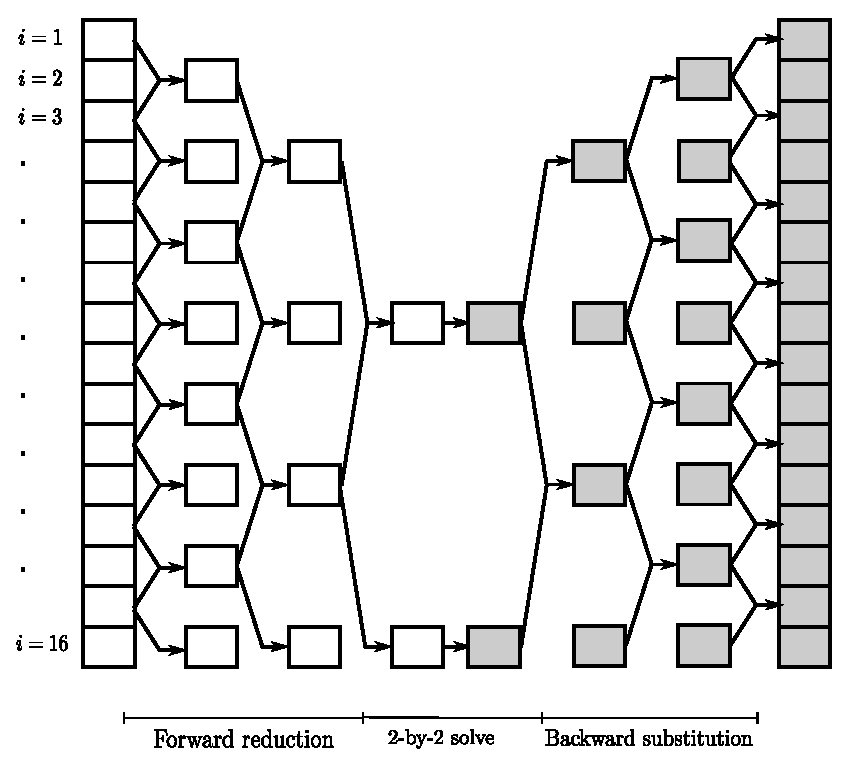
\includegraphics[height=200pt]{img/cyclic-reduction.eps}
\end{center}
\caption{Cyclic reduction -
the values that are solved for at each step of backward reduction
are highlighted}
\label{fig:cyclic-reduction}
\end{figure}

The Cyclic Reduction algorithm consists of two phases:
\emph{forward reduction} and \emph{backward substitution}
(see Figure \ref{fig:cyclic-reduction}).
The forward substitution phase begins with a system of size $n$,
and by expressing every even-indexed equation $i$ as a linear
combination of equations $i$, $i-1$ and $i+1$, reduces it to a
system of size $n/2$.
The process is repeated until a system of 2 equations in 2 unknowns
is left.

For each even-indexed $i$, we define:

\begin{equation*}
k_1 = \frac{a_i}{b_{i-1}},
k_2 = \frac{c_i}{b_{i+1}}
\end{equation*}

Then, we update the values of $a$, $b$, $c$ and $d$ as:

\begin{align} \label{eqn:forward-reduction}
& a^{\prime}_i = -a_{i-1}k_1 & \\
& b^{\prime}_i = b_i - c_{i-1}k_1 - a_{i+1}k_2 & \\
& c^{\prime}_i = -c_{i+1}k_2 & \\
& d^{\prime}_i = d_i - d_{i-1}k_1  - d_{i+1}k_2 &
\end{align}

The 2-by-2 system of equations is solved trivially,
yielding $x_n$ and $x_{n/2}$.
In the backward substitution phase,
every odd-indexed unknown $x_i$ is solved for by
substituting the known values of $x_{i-1}$ and $x_{i+1}$:

\begin{align} \label{eqn:back-substitution}
x_i = \frac{d^{\prime}_i - a^{\prime}_ix_{i-1} - c^{\prime}_ix_{i+1}}{b^{\prime}_i}
\end{align}

At each step, for the last index $i=n$,
the forward reduction step is instead:
\begin{align} \label{eqn:forward-reduction-last}
    & a^{\prime}_n = -a_{n-1}k_1 & \\
    & b^{\prime}_n = b_n - c_{n-1}k_1 & \\
    & d^{\prime}_n = d_n - d_{n-1}k_1 &
\end{align}

And the backward substitution step for $i=1$ is instead:
\begin{align} \label{eqn:back-substitution-first}
x_1 = \frac{d^{\prime}_1 - c^{\prime}_1x_{2}}{b^{\prime}_1}
\end{align}

While cyclic reduction performs far more work per step
compared to the Thomas algorithm,
it is able to solve the system in far fewer steps
on massively parallel architectures.
As pointed out by \cite{Zhang2010FTS},
$n$ parallel processors can solve a tridiagonal system
of size $n$ in $2log(n) - 1$ steps.
The Thomas algorithm, on the other hand,
requires $2n$ steps.

\section{Cyclic reduction for near-Toeplitz systems}

We note from
Equations \ref{eqn:forward-reduction}-\ref{eqn:back-substitution-last}
that each forward reduction step involves 12 operations.
As the LHS matrix is constant,
it is advantageous to pre-compute the coefficients appearing
in the forward reduction step.
For a general tridiagonal matrix,
this requires a substantial amount of storage
(2$n$ for each of the arrays $a$, $b$ and $c$):
$\frac{n}{2} + \frac{n}{4} + \frac{n}{8} + ... = n$
for the reduction steps,
and an additional $n$ for the original coefficients.
\section{Distributed compact-finite difference solution} 

We use the algorithm discussed by Mattor et al.
\cite{mattor1995algorithm}
to distribute and solve the problem among multiple processes. 
We present the algorithm to solve a general tridiagonal system,
and in subsequent sections discuss its adaptation to solving
near-Teoplitz tridiagonal systems on GPUs.

Given a tridiagonal system with  $n$ equations,
to be solved by $P$ processes:

\begin{align}
& \begin{bmatrix}
b_1^p & c_1^p \\
a_2^p & b_2^p & c_2^p \\
      & a_3^p & b_3^p & c_3^p \\
      &       & a_4^p & b_4^p & c_4^p \\
      &       &       &       &  \ddots & c_{m-1}^p\\
      &       &       &       &     a_{m}^p  & b_{m}^p
\end{bmatrix}
\begin{bmatrix}
x_{r,1}^p \\
x_{r,2}^p \\
x_{r,3}^p \\
x_{r,4}^p \\
\vdots \\
x_{r,m}^p
\end{bmatrix}
=
\begin{bmatrix}
r_1^p \\
r_2^p \\
r_3^p \\
r_4^p \\
\vdots \\
r_m^p
\end{bmatrix} & \label{eqn:global-system} 
\end{align}

each process $p$ proceeds by solving the following three ``local''
tridiagonal systems:

\begin{align}
& \begin{bmatrix}
b_1^p & c_1^p \\
a_2^p & b_2^p & c_2^p \\
      & a_3^p & b_3^p & c_3^p \\
      &       & a_4^p & b_4^p & c_4^p \\
      &       &       &       &  \ddots & c_{m-1}^p\\
      &       &       &       &     a_{m}^p  & b_{m}^p
\end{bmatrix}
\begin{bmatrix}
x_{r,1}^p \\
x_{r,2}^p \\
x_{r,3}^p \\
x_{r,4}^p \\
\vdots \\
x_{r,m}^p
\end{bmatrix}
=
\begin{bmatrix}
r_1^p \\
r_2^p \\
r_3^p \\
r_4^p \\
\vdots \\
r_m^p
\end{bmatrix} & \label{eqn:primary-system} \\
%
%
%
& \begin{bmatrix}
b_1^p & c_1^p \\
a_2^p & b_2^p & c_2^p \\
      & a_3^p & b_3^p & c_3^p \\
      &       & a_4^p & b_4^p & c_4^p \\
      &       &       &       &  \ddots & c_{m-1}^p\\
      &       &       &       &     a_{m}^p  & b_{m}^p
\end{bmatrix}
\begin{bmatrix}
u_1^p \\
u_2^p \\
u_3^p \\
u_4^p \\
\vdots \\
u_m^p
\end{bmatrix}
=
\begin{bmatrix}
-a_1^p \\
0 \\
0 \\
0 \\
\vdots \\
0
\end{bmatrix} & \label{eqn:secondary-system-1} \\
%
%
%
& \begin{bmatrix}
b_1^p & c_1^p \\
a_2^p & b_2^p & c_2^p \\
      & a_3^p & b_3^p & c_3^p \\
      &       & a_4^p & b_4^p & c_4^p \\
      &       &       &       &  \ddots & c_{m-1}^p\\
      &       &       &       &     a_{m}^p  & b_{m}^p
\end{bmatrix}
\begin{bmatrix}
l_1^p \\
l_2^p \\
l_3^p \\
l_4^p \\
\vdots \\
l_m^p
\end{bmatrix}
=
\begin{bmatrix}
0 \\
0 \\
0 \\
0 \\
\vdots \\
-c_m^p
\end{bmatrix} & \label{eqn:secondary-system-2}
\end{align}

We call the system in Equation \ref{eqn:primary-system}
the ``primary'' system, and the systems in
Equations
\ref{eqn:secondary-system-1} and \ref{eqn:secondary-system-2}
the ``secondary'' systems.
The local part of the solution to the ``global'' tridiagonal system
(Equation \ref{eqn:global-system})
is obtained as a linear combination of
the solutions to the primary and secondary sytems:

\begin{equation}
    \boldsymbol{x}^p = \boldsymbol{x}_r^p + \
        \alpha^p \boldsymbol{u}^p + \beta^p \boldsymbol{l}^p
    \label{eqn:sum-of-systems}
\end{equation}

where the  parameters $\alpha^p$ and $\beta^p$ are obtained by
solving the following ``reduced'' system of equations:

\begin{equation} \label{eqn:reduced-system}
\begin{bmatrix}
l^1_m & -1 \\
-1    & u^2_1 & l^2_1 \\
      & u^2_m & l^2_m & -1 \\
      &       & -1    & u^3_1 & l^3_1 \\
      &       &       & u^3_m & l^3_n  & -1 \\
      &       &       &       & \ddots & \ddots & \ddots \\
      &       &       &       &        & -1     & u^P_1
\end{bmatrix}
\begin{bmatrix}
\beta^1 \\
\alpha^2 \\
\beta^2 \\
\alpha^3 \\
\beta^3 \\
\vdots \\
\alpha^P
\end{bmatrix}
=
\begin{bmatrix}
x_{r,m}^1 \\
x_{r,1}^2 \\
x_{r,m}^2 \\
x_{r,1}^3 \\
x_{r,m}^3 \\
\vdots \\
x_{r,1}^P \\
\end{bmatrix}
\end{equation}

$P = n/m$ is the number of processes.
We note that the reduced system is sized $2P-2$,
and that its assembly requires communication between the processes.
The general solution procedure is then:

\begin{enumerate}
    \item Each process $p$ solves the primary and secondary systems
        to obtain $\boldsymbol{x}_r^p$, $u^p$ and $l^p$
    \item The ``reduced'' system is assembled and solved for
        the coefficients $\alpha^p$ and $\beta^p$
    \item The local solution is computed from Equation \ref{eqn:sum-of-systems}
\end{enumerate}

\subsection{Evaluation of the right-hand side}

\subsection{Evaluation of the right-hand side}

\subsection{Solution of primary Near-Toeplitz tridiagonal systems}

\subsection{Solution of reduced system}

\subsection{Solution of secondary systems}

\section{Results}

\section*{References}

\bibliography{references}
\bibliographystyle{elsarticle-num}
\end{document}
